\section{Ziele}
\label{sec:ziele}
Es soll zuerst die Bragg Bedingung an einem LiF Kristall überprüft werde.
Außerdem soll im Experiment das Kupfer Röntgenspektrum gemessen, dargestellt und analysiert werden.
Im letzten teil des Versuchs soll die Absorption von verschiedenen Metallen untersucht werden.
\section{Theoretische Grundlagen}
\label{sec:theorie}

\subsection{Erzeugung von Röntgenstrahlung}
Um Bremsstrahlung zu erzeugen wird mit einer evakuierten Röhren mit einem Glühdraht als Kathode und einer Metallanode gearbeitet.
Aus dem Glühdraht werden Elektronen ausgelöst und mit einer Beschleunigungsspannung zur Anode hin beschleunigt.
Wenn die ausgelösten Eleltronen auf die Anode treffen wird Röntgenstrahlung erzeugt und in Richtung einer Probe gelenkt.
Die Röngtgenstrahlung die bei diesem Versuchsaufbau erzeugt wird hat ein spezielles Spektrum, das aus einem kontinuierlichen Bremsberg und chrakteristischen Peaks besteht.
\subsubsection{Bremsspektrum}
Wenn die Elektronen aus der Glühkathode in das Anodenmaterial eindringen, wirkt die Coulombanziehung auf die Elektronen und sie werden abgelenkt und geben EM strahlung ab,wodurch sie auch abgebremst werden.
Da die Elektronen kontinuierlich abgebremst werden entsteht auch ein kontinuierliches Bremsspektrum.
Das kontinuierliche Bremsspektrum hat dabei die Form eines sogenannten Bremsberg, wie in Abb \ref{fig:Bremsspektrum} gut zu erkennen.
\begin{figure}
    \centering
    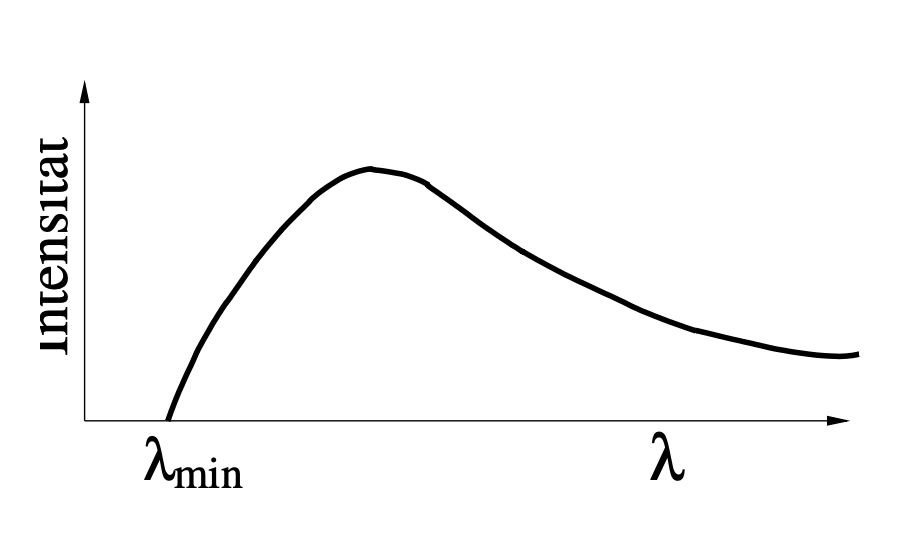
\includegraphics[width=0.7\textwidth]{bilder/Bremsspektrum.png}
    \caption{Skizze eines Graphen der die Intensität der Röntgenstrahlung in abhängigkeit von der Wellenlänge zeigt. (Quelle \cite{Anleitung})}
    \label{fig:Bremsspektrum}
\end{figure}
Der Bremsberg entsteht, da die Elektronen maximal die gesamte kinetische Energie abgeben können.
Die daraus resultierende minimale Wellenlänge lässt sich mithilfe der Beschleunigungsspannung berechnen (Gl. \ref{eqn:E_kin_min}).
Dass der Bremsberg vor seinem Maximum nicht unmittelbar auf Null abflacht, ist damit zu erklären, dass das Messinstrument Strahlung unter einem Grenzwert nicht mehr detektieren kann.
Das Maximum des Bremsbergs entspricht der Wellenlänge an der die Elektronen ihre gesamte kinetische Energie abgeben. Der Berg flacht von da aus immer weiter ab und nähert sich der y-Achse immer weiter an.
\begin{equation}
    \lambda_{\text{min}} = \frac{hc}{e_0 U} \label{eqn:E_kin_min}
\end{equation}
\subsubsection{Charakteristische Peaks}
Neben dem Bremsspektrum entstehen im Spektrum auch noch Peaks die für das jeweilige Anodenmaterial charakteristisch sind.
Die charakteristischen Peaks entstehen dadurch, dass das Anodenmaterial durch die Elektronen ionisiert wird und dabei eine bestimmte Energie emittiert.
Bei der Ionistation eines Atoms wird ein Platz in einer der Schalen des Atoms,mit der Energie $E_{\text{n}}$, frei und kann durch ein Elektron aus einer höheren Schale mit der Energie $E_{\text{m}}$ besetzt werden.
Wenn ein Elektron aus einer höheren Schale in einen freien Platz in einer energetisch günstigeren Schale wechselt, dann gibt es dabei die Energiedifferenz $\Delta E = E_{\text{m}} -E_{\text{n}}$ in Form von Röntgenstrahlung ab.
\begin{description}
    \item[Benennung der Übergänge]
    Wenn man die spezielle Strahlung benennen möchte muss man zum einen die Schale aus der das Elektron kommt, aber auch die Schale in die es wechselt angegeben werden.
    Die Schalen eines Atoms werden mit den Großbuchstaben ab K (K,L,M,...) bezeichnet und bezeichnen beim Schalenwechsel die Ziel Schale.
    Um zu bestimmen aus welcher Schale das Elektron stammt wird der Bezeichnung der Zielschale noch ein Index hinzugefügt mit einem entsprechenden griechischen Buchstaben.
    Wenn ein Elektron aus der nächst höheren Schale kommt wird es mit $\alpha$ bezeichnet und die Schalen danach mit den entsprechenden höheren Buchstaben($\alpha,\beta,\gamma,...$).
    Wenn ein Elektron nun zum Beispiel aus der L in die K Schale wechselt wird dieser Übergang mit $K_{\alpha}$ bezeichnet.
\end{description}
Um die Energie der Elektronen auf den verschiedenen Schalen zu bestimmen ist es allerdings stark vereinfacht, wenn nur die Coulombanziehung des Kerns betrachtet wird.
Damit die sich die Energie der realen Energie der Elektronen weiter annähert,werden in diesem Experiment zusätzlich die Elektronen in den Schalen zwischen dem Kern und dem zu betrachtenden Elektron mit einberechnet.
Durch diese Elektronen ist die Kernladung weiter abgeschwächt und für die Bindungsenergie der äußeren Schalen ergibt sich \ref{eqn:Bindungsenergie}
\begin{equation}
    E_{\text{n}} = -R_{\text{y}} z_{\text{eff}}^2 \cdot \frac{1}{n^2} \label{eqn:Bindungsenergie}
\end{equation}
Mit der Rydberg-Energie $R_{\text{y}} = hR = hcR_{\infty}$, aus der Rydberg-Konstanten $R_{\infty} ≈ 1,097 \cdot 10^{7} \text{m}^{-1}$  oder der Rydberg-Frequenz $R$, und der effektiven Kernladungszahl $z_{\text{eff}} = z-\sigma$ die sich aus der Abschirmkonstanten $\sigma$ berechnen lässt.
Damit ergibt sich beispielsweise für den $K_{\alpha}$ Übergang.
\begin{equation*}
    E_{K_{\alpha}}= R_{\text{y}}(z-\sigma_1)^2 \frac{1}{1^2} - R_{\text{y}}
\end{equation*}
Der Abschirmkoeffizient verändert sich dabei für jedes Elektron, ist aber mit empirischen Methoden gut zu bestimmen.
Entgegen der Erwartung sind die charakteristischen Linien allerdings nicht nur an einem genau definierten Punkt zu finden, sondern erstrecken sich über ein Wellenlängenintervall.
Die Breite der Linien ist durch den unterschiedlichen Bahndrehimpuls und Spin der Elektronen zu erklären, und wird dann durch die Auflösung des Messgeräts noch verstärkt.


\subsection{Absorption}
Bei Röntgenstrahlung mit einer Energie von weniger als $1 \text{MeV}$ finden in Materialien hauptsächlich der Compton Effekt und der Photoeffekt statt und die Strahlung wird dementsprechend beim Durchdringen des Materials abgeschwächt.
Dabei ist zu beobachten das der Absorptionskoeffizient für steigende Energie sinkt und Ein Sprung des Abbsorptionskoeffizienten an den Stellen stattfindet, an denen die Photonenenrgie die Bindungsenergie der versiedenen Elektronen übersteigt (\ref{fig:Absorption}).
\begin{figure}
    \centering
    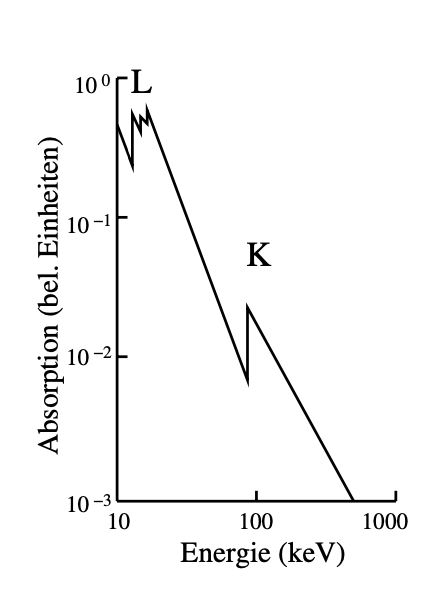
\includegraphics[width=0.3\textwidth]{bilder/Absorption.png}
    \caption{Skizze eines Graphen für das auftragen der Absorption gegen die Energie. Auf der Skizze sind die gut erkenntlichen L und K Kanten beschriftet. (Quelle \cite{Anleitung})}
    \label{fig:Absorption}
\end{figure}
Diese Sprünge des Absorptionskoeffizienten nennt man Absorptionskanten und die Kanten liegen fast genau bei den Energien, die den Bindungsenergien der Elektronen entsprechen.
Es gibt im Absorptionsspektrum  drei verschiedene L-Kanten aber nur eine K-Kante.
Wenn nun zusätzlich die Feinstruktur der Probe berücksichtigt wird lässt sich die Bindungsenergie $E_{\text{n,j}}$ gut mit der Sommerfeldschen Feinstrukturformel (\ref{eqn:Sommerfeldsche_Feinstrukturformel}) bestimmen.
\begin{equation}
    E_{\text{n,j}} = -R_{\text{y}}\left(z_{\text{eff,}1}^2\frac{1}{n^2}+\alpha^2z_{\text{eff,}2}^4\frac{1}{n^3}\left(\frac{1}{j+\frac{1}{2}}-\frac{3}{4n}\right) \right)     \label{eqn:Sommerfeldsche_Feinstrukturformel}
\end{equation}
Mit der Sommerfeldschen Feinstrukturkonstanten $\alpha$, der Hauptquantenzahl $n$ und dem Gesamtdrehimpuls $j$ des Elektrons.
Für die Elektronen aus der K-Schale lässt sich so aus der Feinstrukturformel der Abschirmkoeffizient bestimmen (\ref{eqn:Sigma}).
\begin{equation}
    \sigma_{\text{K}} = Z - \sqrt{\frac{E_{\text{K}}}{R_{\text{y}}}-\frac{\alpha^2Z^4}{4}} \label{eqn:Sigma}
\end{equation}
In der Formel berücksichtigt dabei der Subtrahend in der Wurzel die Feinstrukturspaltung.

\subsection{Bragg Reflexion}
\begin{figure}
    \centering
    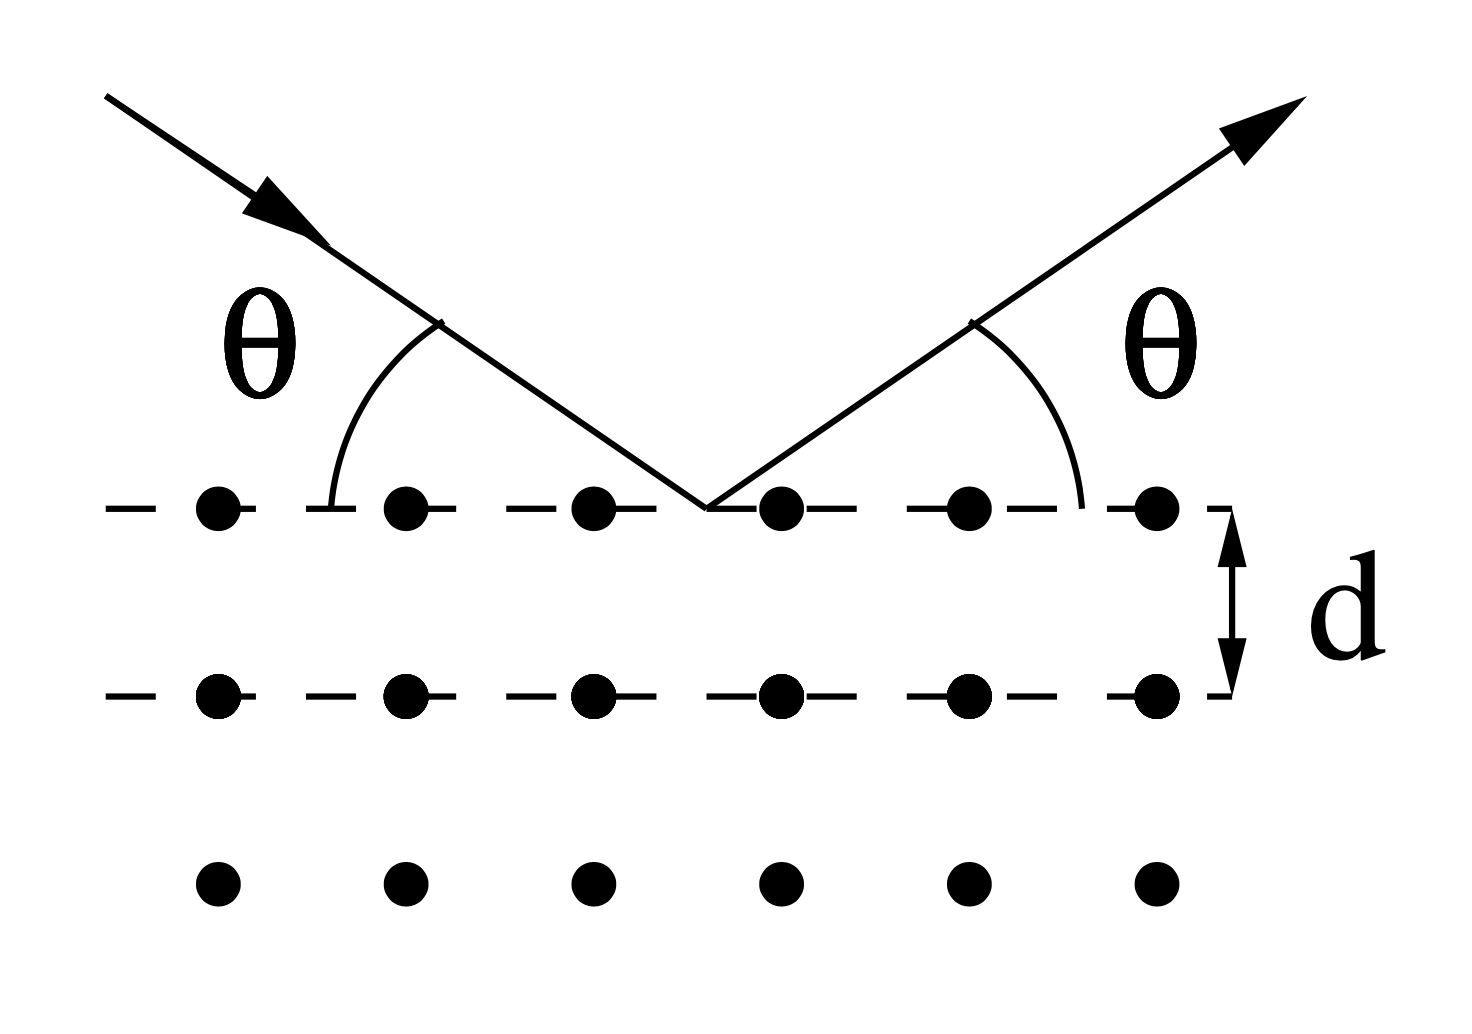
\includegraphics[width=0.5\textwidth]{bilder/Bragg_Reflexion.png}
    \caption{Eine schematische Skizze der Bragg Reflexion. (Quelle \cite{Anleitung}}
    \label{fig:Bragg_Reflexion}
\end{figure}
Als Bragg Reflexion wird der Effekt bezeichnet, der stattfindet wenn elektromagnetische Strahlung auf einen Kristall mit einem regelmäßigen Kristallgitter fällt.
Wenn die EM-Strahlung in einem genau definierten Winkel(\ref{eqn:Bragg_Bedingung}), der vom Kristallgitterabstand und der Wellenlänge der Strahlung abhängt, auf den Kristall fällt, kann sie mit maximaler Intensität reflektiert werden.
Dieses wellenlängeabhängige Phänomen lässt sich dadurch erklären, dass wenn der Gitterabstand ein Vielfaches der Wellenlänge ist, die Strahlung die an zwei verschiedenen Schichten des Materials reflektiert wird danach konstruktiv interferiert.
Wenn Strahlung zwischen zwei Schichten konstruktiv interferiert gilt das für belibige Schichten und somit für das gesamte Material.
Wenn die Strahlung allerdings nicht konstruktiv interferiert kommt ein Anteil destruktiver Interferenz hinzu und die Strahlungsintensität wird für entsprechende Wellenlängen geschwächt.
Für die Bragg Reflexion gilt außerdem, dass wenn der Einfallswinkel gleich dem Ausfallswinkel ist, die maximale Intensität reflektiert wird(\ref{fig:Bragg_Reflexion}).
\begin{equation}
    \theta = \arcsin\left( \frac{n\lambda}{2d}\right) \underset{\lambda = \frac{hc}{E}}{=} \arcsin\left( \frac{n h c}{2dE}\right) \label{eqn:Bragg_Bedingung}
\end{equation}
